% Uebung 40) Lautsprecher nach Brinkmeyer
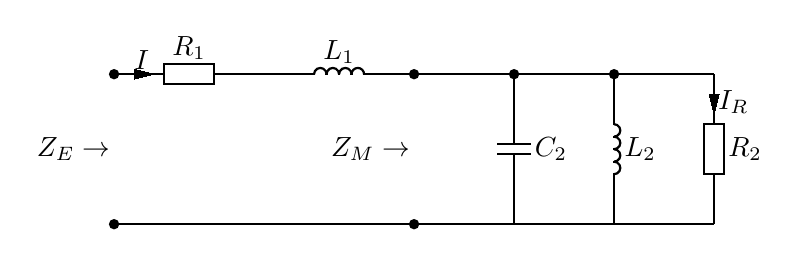
\begin{tikzpicture}[scale=2.54]%
% dpic version 2024.01.01 option -g for TikZ and PGF 1.01
\ifx\dpiclw\undefined\newdimen\dpiclw\fi
\global\def\dpicdraw{\draw[line width=\dpiclw]}
\global\def\dpicstop{;}
\dpiclw=0.8bp
\dpiclw=0.8bp
\dpicdraw[fill=black](0,0) circle (0.007874in)\dpicstop
\dpicdraw[fill=black](0,-0.75) circle (0.007874in)\dpicstop
\draw (0,-0.375) node[left=-2bp]{$ Z_E \rightarrow$};
\dpicdraw (0,0)
 --(0.25,0)\dpicstop
\dpicdraw (0.5,0)
 --(0.5,0.05)
 --(0.25,0.05)
 --(0.25,-0.05)
 --(0.5,-0.05)
 --(0.5,0)\dpicstop
\dpicdraw (0.5,0)
 --(0.75,0)\dpicstop
\draw (0.375,0.05) node[above=-2bp]{$ R_1$};
\filldraw[line width=0bp](0.1,-0.025)
 --(0.2,0)
 --(0.1,0.025) --cycle\dpicstop
\dpicdraw (0.177094,0)
 --(0.1,0)\dpicstop
\draw (0.138547,0) node[above=-2bp]{$ I$};
\dpicdraw (0.75,0)
 --(1,0)\dpicstop
\dpicdraw (1,0)
 --(1,-0.005556)\dpicstop
\dpicdraw (1,-0)
 ..controls (1,0.011165) and (1.005956,0.021481)
 ..(1.015625,0.027063)
 ..controls (1.025294,0.032646) and (1.037206,0.032646)
 ..(1.046875,0.027063)
 ..controls (1.056544,0.021481) and (1.0625,0.011165)
 ..(1.0625,0)\dpicstop
\dpicdraw (1.0625,0)
 --(1.0625,-0.005556)\dpicstop
\dpicdraw (1.0625,-0)
 ..controls (1.0625,0.011165) and (1.068456,0.021481)
 ..(1.078125,0.027063)
 ..controls (1.087794,0.032646) and (1.099706,0.032646)
 ..(1.109375,0.027063)
 ..controls (1.119044,0.021481) and (1.125,0.011165)
 ..(1.125,0)\dpicstop
\dpicdraw (1.125,0)
 --(1.125,-0.005556)\dpicstop
\dpicdraw (1.125,-0)
 ..controls (1.125,0.011165) and (1.130956,0.021481)
 ..(1.140625,0.027063)
 ..controls (1.150294,0.032646) and (1.162206,0.032646)
 ..(1.171875,0.027063)
 ..controls (1.181544,0.021481) and (1.1875,0.011165)
 ..(1.1875,0)\dpicstop
\dpicdraw (1.1875,0)
 --(1.1875,-0.005556)\dpicstop
\dpicdraw (1.1875,0)
 ..controls (1.1875,0.017259) and (1.201491,0.03125)
 ..(1.21875,0.03125)
 ..controls (1.236009,0.03125) and (1.25,0.017259)
 ..(1.25,0)\dpicstop
\dpicdraw (1.25,0)
 --(1.25,-0.005556)\dpicstop
\dpicdraw (1.25,0)
 --(1.5,0)\dpicstop
\draw (1.125,0.03125) node[above=-2bp]{$ L_1$};
\dpicdraw[fill=black](1.5,0) circle (0.007874in)\dpicstop
\dpicdraw[fill=black](1.5,-0.75) circle (0.007874in)\dpicstop
\draw (1.5,-0.375) node[left=-2bp]{$ Z_M \rightarrow$};
\dpicdraw (1.5,0)
 --(2,0)\dpicstop
\dpicdraw[fill=black](2,0) circle (0.007874in)\dpicstop
\dpicdraw (2,0)
 --(2,-0.35)\dpicstop
\dpicdraw (1.916667,-0.35)
 --(2.083333,-0.35)\dpicstop
\dpicdraw (1.916667,-0.4)
 --(2.083333,-0.4)\dpicstop
\dpicdraw (2,-0.4)
 --(2,-0.75)\dpicstop
\draw (2.083333,-0.375) node[right=-2bp]{$ C_2$};
\dpicdraw (2,0)
 --(2.5,0)\dpicstop
\dpicdraw[fill=black](2.5,0) circle (0.007874in)\dpicstop
\dpicdraw (2.5,0)
 --(2.5,-0.25)\dpicstop
\dpicdraw (2.5,-0.25)
 --(2.494444,-0.25)\dpicstop
\dpicdraw (2.5,-0.25)
 ..controls (2.511165,-0.25) and (2.521481,-0.255956)
 ..(2.527063,-0.265625)
 ..controls (2.532646,-0.275294) and (2.532646,-0.287206)
 ..(2.527063,-0.296875)
 ..controls (2.521481,-0.306544) and (2.511165,-0.3125)
 ..(2.5,-0.3125)\dpicstop
\dpicdraw (2.5,-0.3125)
 --(2.494444,-0.3125)\dpicstop
\dpicdraw (2.5,-0.3125)
 ..controls (2.511165,-0.3125) and (2.521481,-0.318456)
 ..(2.527063,-0.328125)
 ..controls (2.532646,-0.337794) and (2.532646,-0.349706)
 ..(2.527063,-0.359375)
 ..controls (2.521481,-0.369044) and (2.511165,-0.375)
 ..(2.5,-0.375)\dpicstop
\dpicdraw (2.5,-0.375)
 --(2.494444,-0.375)\dpicstop
\dpicdraw (2.5,-0.375)
 ..controls (2.511165,-0.375) and (2.521481,-0.380956)
 ..(2.527063,-0.390625)
 ..controls (2.532646,-0.400294) and (2.532646,-0.412206)
 ..(2.527063,-0.421875)
 ..controls (2.521481,-0.431544) and (2.511165,-0.4375)
 ..(2.5,-0.4375)\dpicstop
\dpicdraw (2.5,-0.4375)
 --(2.494444,-0.4375)\dpicstop
\dpicdraw (2.5,-0.4375)
 ..controls (2.511165,-0.4375) and (2.521481,-0.443456)
 ..(2.527063,-0.453125)
 ..controls (2.532646,-0.462794) and (2.532646,-0.474706)
 ..(2.527063,-0.484375)
 ..controls (2.521481,-0.494044) and (2.511165,-0.5)
 ..(2.5,-0.5)\dpicstop
\dpicdraw (2.5,-0.5)
 --(2.494444,-0.5)\dpicstop
\dpicdraw (2.5,-0.5)
 --(2.5,-0.75)\dpicstop
\draw (2.53125,-0.375) node[right=-2bp]{$ L_2$};
\dpicdraw (2.5,0)
 --(3,0)\dpicstop
\dpicdraw (3,0)
 --(3,-0.25)\dpicstop
\dpicdraw (3,-0.5)
 --(3.05,-0.5)
 --(3.05,-0.25)
 --(2.95,-0.25)
 --(2.95,-0.5)
 --(3,-0.5)\dpicstop
\dpicdraw (3,-0.5)
 --(3,-0.75)\dpicstop
\draw (3.05,-0.375) node[right=-2bp]{$ R_2$};
\filldraw[line width=0bp](2.975,-0.1)
 --(3,-0.2)
 --(3.025,-0.1) --cycle\dpicstop
\dpicdraw (3,-0.177094)
 --(3,-0.1)\dpicstop
\draw (3,-0.138547) node[right=-2bp]{$ I_R$};
\dpicdraw (3,-0.75)
 --(0,-0.75)\dpicstop
\end{tikzpicture}%
